\chapter{Some LaTeX and RaM Report Template Showcasing}
\label{ch:one}
This is a demo chapter designed to show-case the elements frequently used in reports.

References to the bibliography:

\begin{itemize}
	\item A normal reference:  $\backslash$citep\{\} results in: \citep{foo}
	\item A textual reference: $\backslash$citet\{\} results in: \citet{foo}
	\item Multiple references: $\backslash$citep\{foo,bar\}  results in:
	\citep{foo,bar}
\end{itemize}

Remember to run bibtex on the report.tex file in order to generate the actual
bibliography.

References to other parts of the document can be made as well by using
$\backslash$ref\{app:one\}, which resuls in:\\ \ref{app:one} (only the number).

Because we are using the Latex Hyperref package, you can also use $\backslash$autoref\{app:one\}, which results in:\\ \autoref{app:one} (reference name and number).

\section{This is a section}
This is a section in the report
Some references to have a couple of bibliography items to check the bibtex
formatting: 20-sim \citep{20sim}, \citep{DesignTraject}, \citep{CTlib},
\citep{gCSP} and \citep{Hoare}

\subsection{This is a subsection}
This is an itemize environment.

\begin{itemize}
	\item cedoctype	
	\item atbeginend
\end{itemize}

This is an enumerate environment.

\begin{enumerate}
	\item cedoctype	
	\item atbeginend
\end{enumerate}

This is an nested and mixed enumerate/enumerate/itemize environment

\begin{enumerate}
	\item Lorem
		\begin{enumerate}
			\item dolor
			\item vel
				\begin{itemize}
					\item foo
					\item bar	
				\end{itemize}
			\item sollicitudin
		\end{enumerate}
	\item Ipsum
		\begin{enumerate}
			\item egestas
			\item blandit
			\item lectus
		\end{enumerate}
\end{enumerate}

These were the most used list environments.

\newpage
\subsubsection{This is a subsubsection}
When using code use the lstlisting environment

\begin{lstlisting}
	int someFunction( void ) 
	{
		int foo, bar;

		foo = 0;
		bar = 10;

		foo += bar;

		return true;
	}
\end{lstlisting}

You can also use tables (like Table \ref{tab:demotab}):

\begin{table} [h!]
	\begin{tabular}{l|c|r}
		This &is &the head\\
		\hline
		This 	&is 	&content\\
		and 	&some 	&more\\
	\end{tabular}
	\caption{Use caption to elaborate}
	\label{tab:demotab}
\end{table}

Or insert a figure (referenced with \ref{fig:demofig}).

\begin{figure}[h!t]
	\begin{center}
		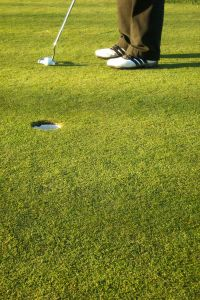
\includegraphics[height=60mm]{images/demo.png}
	\end{center}
	\caption{Figures can have a caption too}
	\label{fig:demofig}
\end{figure}

\section{Rich Report Outline}
The template offers a set of commands to easily create and maintain a Rich Report Outline (RRO) of a document.
The set of commands can be used to insert special RRO items and using a prebuild \LaTeX{} file, the RRO items can be converted into a RRO document.
The commands also could help an author remembering \textit{action points} and his/her supervisor what new action points should be read and which parts did not change since last review.
So using the RRO package is a good thing for everyone!
More information about RROs can also be found on the CE wiki: \url{http://cewiki.ewi.utwente.nl/wiki/index.php/Report_Writing}

\subsection{RRO commands}
First the $\backslash$rro\{rro item\} command.
It can be used to create some comments about a section (for example to describe what should be explained in the different sections).
The result is:
\rro{This is a default rro item with some text}

Multi line texts, containing all kinds of \LaTeX{} commands are also supported:\par
\rro{\begin{itemize}
	  \item A bulleted list is also supported
	  \item (Also with more than one bullet)
	  \item Other special commands are supported as well:
	  \item Citation: \citep{foo}, styles: \textbf{bold} / \textit{italic}
	\end{itemize}}
\rro{And now citation outside an itemize environment: \cite{bar}}

We have also the $\backslash$rrotodo\{rro item\} command (or abbreviated:
$\backslash$rrot\{rro item\}), it can be used for action points. The result
is:\par
\rrotodo{This is a rro item with a todo status}
\rrot{This is a second rro item with a todo status}

We have also the $\backslash$rrowip\{rro item\} command (or abbreviated:
$\backslash$rrow\{rro item\}), it can be used for work in progress. The result
is:\par
\rrowip{This is a rro item with a work in progress status}
\rrow{This is a second rro item with a work in progress status}

We have also the $\backslash$rrodone\{rro item\} command (or abbreviated:
$\backslash$rrod\{rro item\}). After you have
finished an action point, you could use this command to indicate it is done and needs
reviewing by your supervisor. The result is:\par
\rrodone{This is rro item with a done status}
\rrod{This is a second rro item with a done status}

We have also the $\backslash$rrogone\{rro item\} command (or abbreviated:
$\backslash$rrog\{rro item\}). The result is still
visible in the DVI output, but gone in the PDF version. It also is visible in
the RRO document itself, so a complete RRO always is available. It can be used
after your supervisor has read the done action point and not further actions
are required. (Otherwise, if new actions are required you could set it to todo 
again) The result is\ifpdf\ldots Empty since this is a PDF!\else :\par\fi
\rrogone{This item is not visible in the pdf version}
\rrog{This is a second item that is not visible in the pdf version}

RRO items also can used as bulleted lists, eg for sub RRO items. 
$\backslash$rroi, $\backslash$rroit, $\backslash$rrod and $\backslash$rrow $\backslash$rrog can
be used for these sub rro items. It results in:

\rroi{A bulleted rro item is also supported}
\rroit{(which can contain the different RRO item types)}
\rroid{(of which some are done)}
\rroiw{(and these ones are work in progress)}
\rroig{(and others are gone)}

\subsection{The resulting RRO document}
In order to build a Rich Report Outline document run the BuildRRO.bat file or
use \textit{make rro} on non-Windows systems.

After building the document, this section would result in:\\
% Quite hard to use the RichReportOutline.rro file while it is being build
% So fake a RRO (grabbed from RichReportOutline.rro):
\rroaddsection{section}{1.2}{Rich Report Outline}
\rroaddsection{subsection}{-}{RRO commands}
\rroaddline{rro}{This is a default rro item with some text}
\rroaddline{rro}{\begin {itemize} \item A bulleted list is also supported \item (Also with more than one bullet) \item Other special commands are supported as well: \item Citation: \citep {foo}, styles: \textbf {bold} / \textit {italic} \end {itemize}}
\rroaddline{rro}{And now citation outside an itemize environment: \cite {bar}}
\rroaddline{todo}{This is a rro item with a todo status}
\rroaddline{todo}{This is a second rro item with a todo status}
\rroaddline{inpr}{This is a rro item with a work in progress status}
\rroaddline{inpr}{This is a second rro item with a work in progress status}
\rroaddline{done}{This is rro item with a done status}
\rroaddline{done}{This is a second rro item with a done status}
\rroaddline{gone}{This item is not visible in the pdf version}
\rroaddline{gone}{This is a second item that is not visible in the pdf version}
\rroaddline{rroi}{A bulleted rro item is also supported}
\rroaddline{rroit}{(which can contain the different RRO item types)}
\rroaddline{rroid}{(of which some are done)}
\rroaddline{rroig}{(and others are gone)}

In order to remove \textit{all} output from the RRO commands in a document, use\\[3pt]
$\backslash$usepackage\textbf{[final]}\{rro\}\\[3pt]
(the line to modify can be found in include$\backslash$preamble.tex of this template.)\\
\textbf{Note}: The information to build the RRO document itself is still being collected, so this functionality is not broken when using the \textit{final} parameter.

\section{Notes commands}
This template has the $\backslash$note\{Some comments\} command.
The result is:\par
\note{Some comments}

This template has the $\backslash$notedone\{Some comments\} command.
The result is:\par
\notedone{Some comments}

This template has the $\backslash$notegone\{Some comments\} command.
The result is:\par
\notegone{This item is not visible in the pdf version}

This template has the $\backslash$sidenote\{The comment goes here\} command.
The result is written in the outer page margin.\par
\sidenote{The comment goes here}

In order to remove \textit{all} output from the Notes commands in a document, use\\[3pt]
$\backslash$usepackage\textbf{[final]}\{notes\}\\[3pt]
(the line to modify can be found in include$\backslash$preamble.tex of this template.)

\section{Requirement commands}
The template contains a requirements package (very new, so it might/still need to polishing), with it you can easily state some requirements:

\requirement{req:command}{The $\backslash$requirement command must define the requirement.}
The requirement description/explanation can follow each requirement.

\requirement{req:label}{The requirements must have labels}
So it is possible to refer back to the requirement.
For example by using the $\backslash$autoref command, like this: This shows that \autoref{req:label} is implemented!

\subrequirement{req:sub}{Sub requirements should also be available}
So it is possible to further specify the requirements.

\subrequirement{req:user}{users of this package should provide bug reports}
Otherwise the package stays `very new' and never matures\ldots

\subsection{Known issues}
Thiis are the known issues (make sure to circumvent them!):
\begin{itemize}
\item When a requirement is at the bottom of the page, its description might start on the next page. Both the requirements and 9at least) the first line of the description should be on the same page (see \autoref{req:command} in the current example document)
\end{itemize}

\section{Draft and Final versions}
The template supports draft and final versions. The first two lines in document.tex can be used to switch between the draft and final versions. The draft version adds
\begin{itemize}
\item line numbers to easy discussions with supervisors/reviewers
\item support for RRO and notes package
\item the text (Draft) and dates in the headers/footers
\end{itemize}

\section{Symbols}
\subsection{Accent symbols}
\'{a} \`{a} \"{a} \^{a} \~{a}
\c{c} \={a} \o \`{A}

The command for the circular degree symbol is \$ $\hat{}$\{$\backslash$circ\}\$
which results in $^{\circ}$.\\
The command for the euro symbol (\euro) is $\backslash$euro. To get a correct
unbreakable spacing between the symbol and the value use
$\backslash$euro\{value\}, which results in \euro{10}.

\section{Super and subscript}
The superscript command is $^{characters to be superscripted}$.

Subscripts

The subscript command is $_{characters to be subscripted}$.

